\documentclass{beamer}
\usetheme{Malmoe}
\usepackage[polish]{babel}
\usepackage[utf8]{inputenc}
\usepackage[T1]{fontenc}
\usepackage{wrapfig}
\title{Moja pierwsza prezentacja w Beamer}
\author{Aleksandra Ostrowska}
\date{2024 rok}
\begin{document}
\begin{frame}
\titlepage
\end{frame}

\begin{frame}{Będzie to prezentacja o matematyce dyskretnej}
Bedzie to bardzo interesujące, zapraszam do lektury.
\end{frame}

\begin{frame}{Suma i Iloczyn}
Sprawdzić prawdziwość poniższych równać dla podanych wartości zmiennych, obliczając wartość lewej i prawej strony.
\begin{enumerate}[a)]
\item $\sum_{i=1}^{n}i=(1+n)n/2$ dla n=3 i n=6\\
$\sum_{i=1}^{3}i=1+2+3=6$, $(1+3)3/2=12/2=6, prawdziwe$\\
$\sum_{i=1}^{6}i=6+4+5+6=21$, $(1+6)6/2=42/2=21, prawdziwe$
\pause
\item $\prod_{1<=i<=5}i^{2}=(5!)^2$\\
$1^{2}*2^{2}*3^{2}*4^{2}*5^{2}=(1*2*3*4*5)^{2}=(5!)^2, prawdziwe$ \cite{Dyskretna}
\end{enumerate}
\end{frame}

\begin{frame}{Zagnieżdżona suma}
Oblicz:
\begin{enumerate}[a)]
\item $\sum_{i=1}^{5}\sum_{j=1}^{5}i+j=\sum_{i=1}^{5}(5i+1+2+3+4+5)=\sum_{i=1}^{5}(5i+15)=\sum_{i=1}^{5}5(i+3)=5(5*3+1+2+3+4+5)=5*(15+15)=5*30=150$
\pause 
\item $\sum_{j=1}^{5}\sum_{i=1}^{5}i+j=\sum_{i=1}^{5}\sum_{j=1}^{5}i+j=150$
\end{enumerate}
\end{frame}

\begin{frame}{Zagnieżdżony iloczyn w sumie i na odwrót}
Oblicz:
\begin{enumerate}[a)]
\item  $\sum_{i=1}^{3}\prod_{j=1}^{3}j^i=\sum_{i=1}^{3}(1*2^{i}*3^{i})=6+6^{2}+6^{3}=6+36+216=258$
\pause
\item  $\prod_{j=1}^{3}\sum_{i=1}^{3}j^i=\prod_{i=1}^{3}(j+j^{2}+j^{3})=\prod_{i=1}^{3}j(1+j+j^2)=(1+1+1)2(1+2+4)3(1+3+9)=3*2*3*7*13=$1683
\end{enumerate}
\end{frame}

\begin{frame}{Działania na zbiorach}
Różnica symetryczna
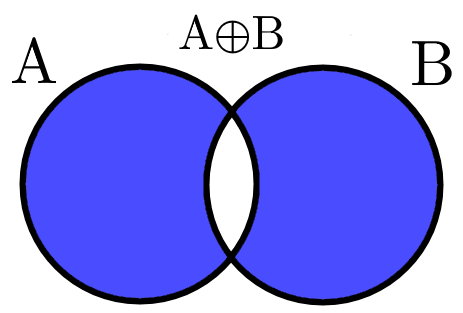
\includegraphics{różnica_symetryczna}\cite{niebezpieczna}\\
Dla A = \{1,2,3\} i B = \{2,4\} \\
$A\oplus B=\{1,3,4\}$
\end{frame}

\begin{frame}{Symmetric difference of 3 sets}
Różnica symetryczna 3 zbiorów
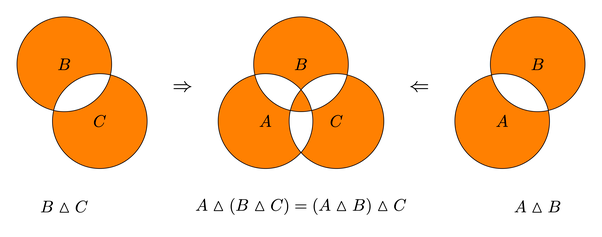
\includegraphics[scale=0.9]{symetryczna3}\cite{r3}\\
Dla A = \{1,2,3,4,5\}, B = \{1,3,5,7\}  i  C= \{4,5,6,7,8\}
$A\oplus B\oplus C=\{5,2,8\}$
\end{frame}

\begin{frame}{Dopełnienie zbioru, Uniwersum}
The complement of set A, denoted by A’, is the set of all elements in the Universal Set that are not in A.\\
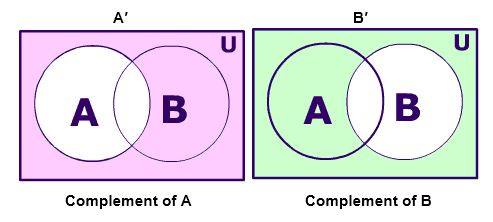
\includegraphics[scale=0.8]{complement}\cite{U}\\
Dla A = \{1,2,3\} i U = \{1,2,3,4,5,6,7\} \\
A'=\{4,5,6,7\}
\end{frame}

\begin{frame}{Dopełnienie zbioru, iloczyn zbiorów (osobno)}
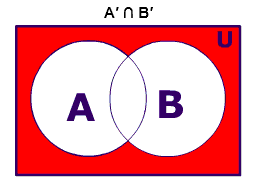
\includegraphics{uOsobno}\\
Dla A = \{1,2,3,4,5\}, B = \{1,3,5,7\}  i U = N \\
$A'\cap B'=N-$ \{1,2,3,4,5,7\}
\end{frame}

\begin{frame}{Dopełnienie zbioru, iloczyn zbiorów (razem)}
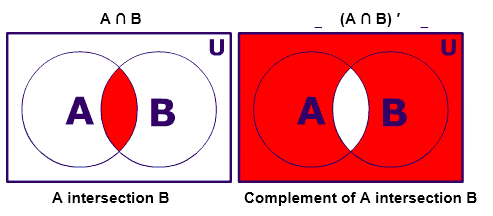
\includegraphics[scale=0.9]{uRazem}\\
Dla A = \{1,2,3,4,5\}, B = \{1,3,5,7\}  i U = N \\
$(A\cap B)'=N-$ \{1,3,5\}
\end{frame}

\begin{frame}{Prawa De Morgana}
\begin{tabular}{l|l}
Nazwa Prawa po angielsku & Expressed in Boolean algebra: \\ \hline 
De Morgan’s Law of Union & $ (A \cup B)' = A' \cap B' $ \\
 De Morgan’s Law of Intersection &  $(A \cap B)' = A' \cup B'$ \\
\end{tabular}
\end{frame}

\begin{frame}{Prawa De Morgana}
\begin{thebibliography}{3}
\bibitem{Dyskretna} Dyskretna \href{https://inf.ug.edu.pl/~zylinski/dydaktyka/}{Matematyka}
\bibitem{niebezpieczna} Różnica symetryczna \href{https://wojcienty.com/artykul/7/matematyka/zbiory/}{warning}
\bibitem{r3} Różnica \href{https://www.quora.com/How-do-you-show-that-the-symmetric-difference-is-associative-for-any-three-sets-A-B-C}{3 zbiorów}
\bibitem{U} Dopełnienie zbioru \href{https://www.askiitians.com/iit-jee-algebra/set-relations-functions/set-theory/complement-of-a-set/}{Universum}
\end{thebibliography}
\end{frame}

\end{document}